\section{Project specifications and hardware}
\label{sec:project_specifications}

\subsection{Distress beacon specifications}

The aim of this project is to build an emergency beacon that is capable of sending three types of distress signals, as shown in Figure~\ref{fig:distress_beacon}: 
\begin{enumerate}
	\item a luminous signal sending morse code; 
	\item an audio signal sending morse code; 
	\item a visual flag type signal sending semaphore code. 
\end{enumerate}
Morse code is a succession of short and long luminous or audio signals, which can describe the letters of the alphabet. Semaphore code uses two flags to describe the different letters of the alphabet. Different inputs will be used to allow different functionalities of the distress beacon. 

\begin{figure}[h]
	\centering
	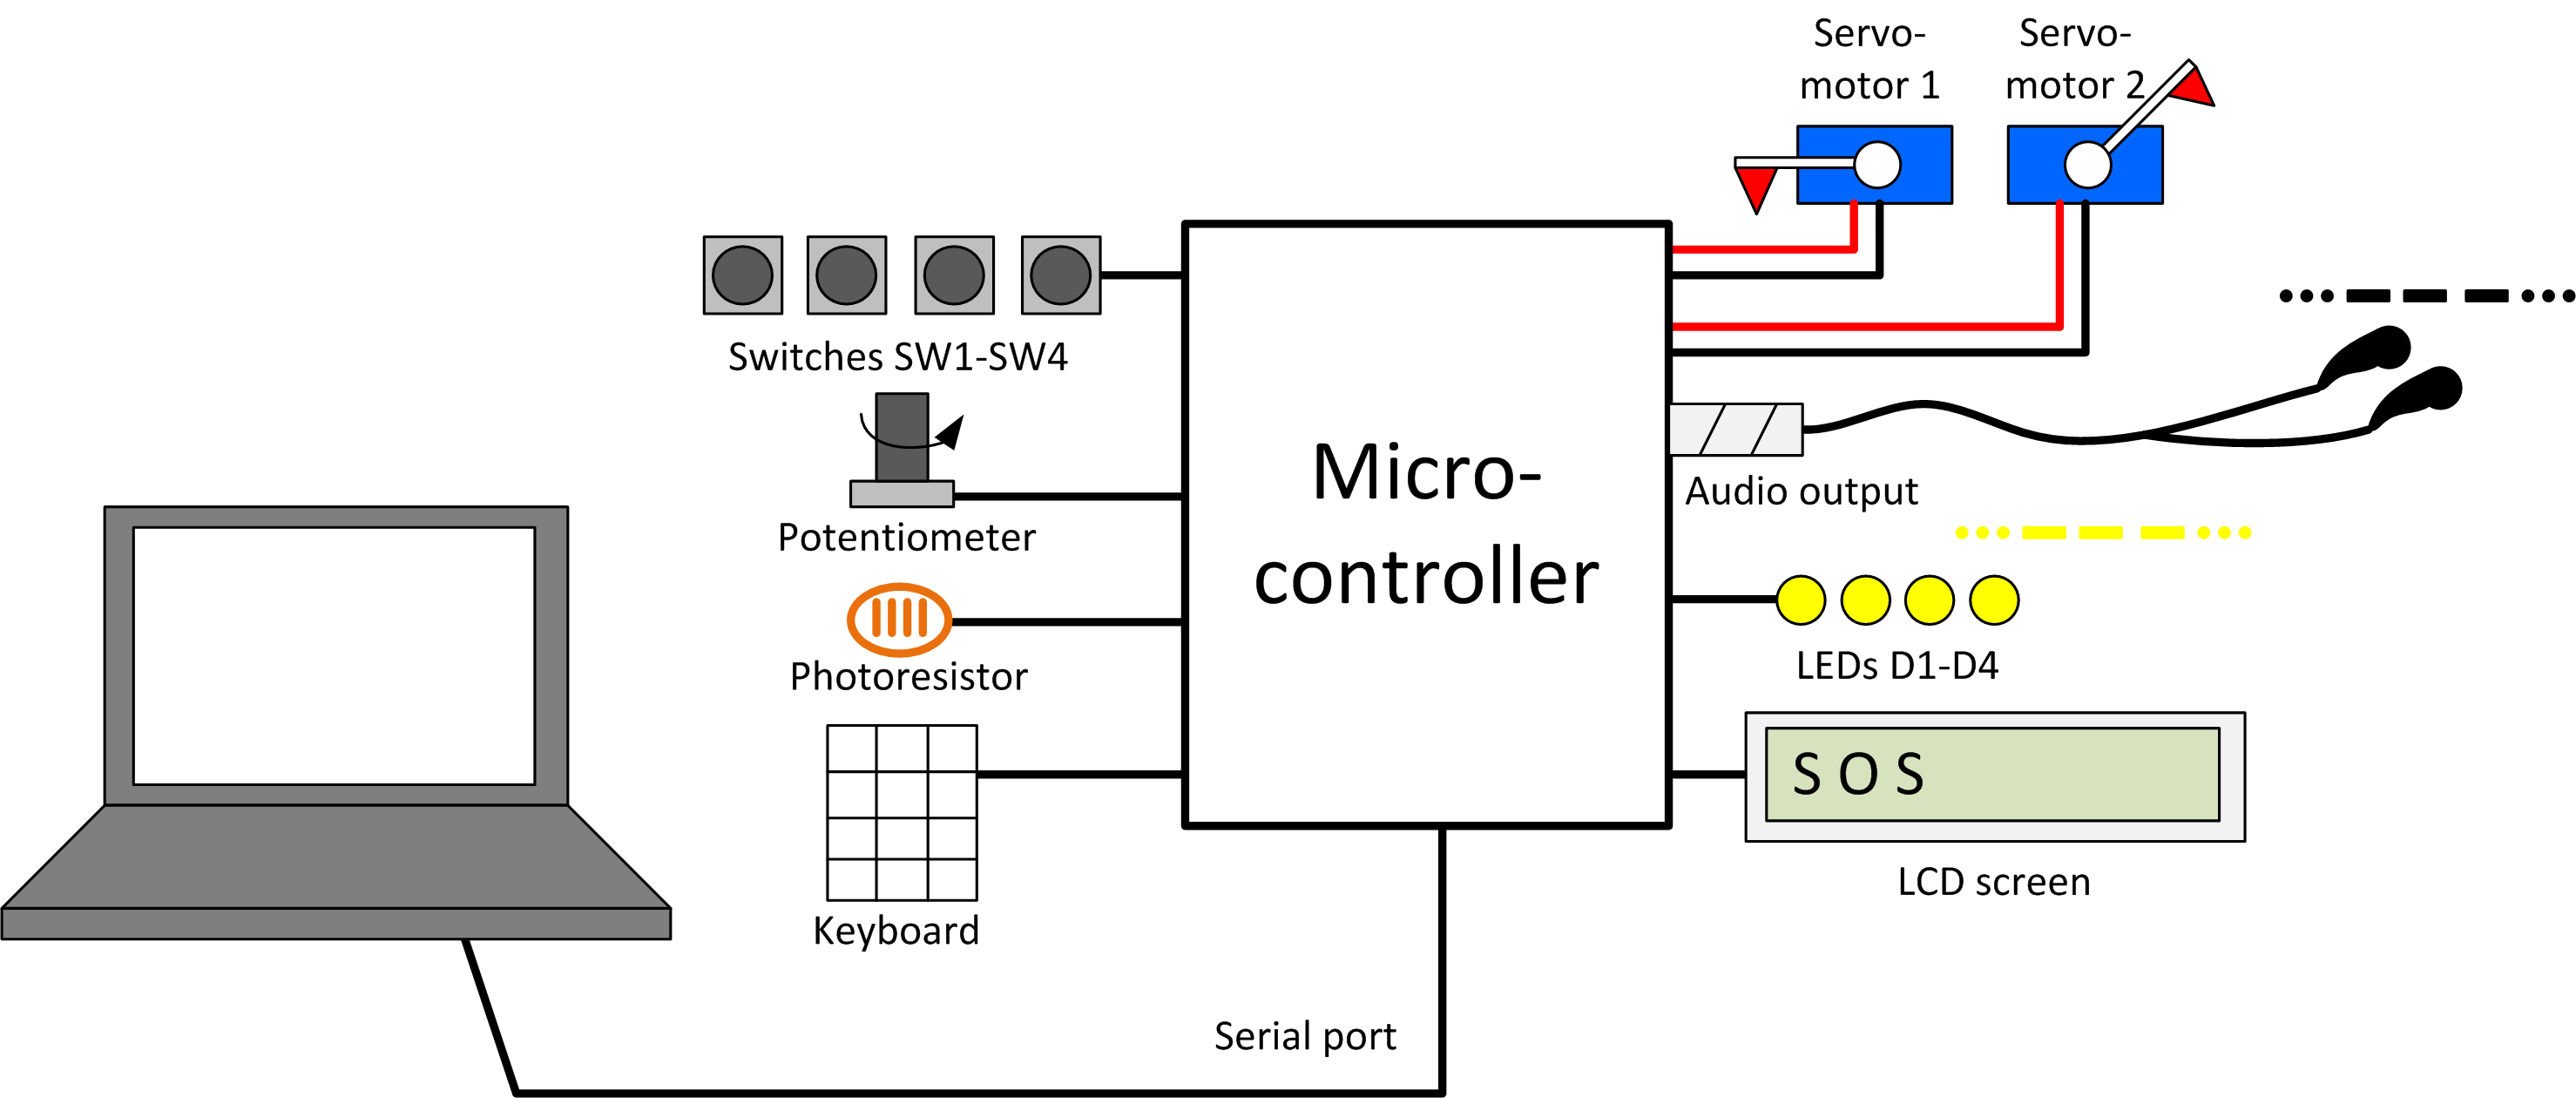
\includegraphics[width=5in]{distress_beacon.png}
	\caption{Schematic representation of the distress beacon inputs and outputs. }
	\label{fig:distress_beacon}
\end{figure}

The inputs are configured as follows. 
\begin{itemize}
	\item \textbf{SW1:} When pressing switch SW1, the LEDs should light up and the audio output should emit a sound as long as the switch is pressed. When the switch is unpressed, the LEDs should go out and the audio output should stop emitting a sound. 
	\item \textbf{SW2:} When pressing switch SW2, the LEDs and audio output should emit a short morse signal. The short morse signal should be 250~ms long. 
	\item \textbf{SW3: } When pressing switch SW3, the LEDs and audio output should emit a long morse signal. The long morse signal should be 500~ms long. 
	\item \textbf{SW4 and Pot: } When turning the potentiometer (Pot), the flag should be going up according to the turning of the potentiometer. When pressing SW4, we change the flag that is controlled with the potentiometer. 
	\item \textbf{Photoresistor: } The photoresistor can detect whether there is ambient light or not. When there is light, only the audio output and semaphore flags should be active. When there is no light, only the audio output and the LEDs should be active. 
	\item \textbf{Keyboard: } We can use the keyboard to send a series of pre-recorded message. For example, pressing ``1'' and ``*'' should start sending ``SOS'' in morse and semaphore code. Pressing ``2'' and ``*'' should send ``BEAMS'' in morse and semaphore code. Other messages are for you to chose. 
	\item \textbf{Serial port: } The user computer can send ASCII characters through the serial port, which are then sent in morse and semaphore code by the distress beacon. The microcontroller also sends two types of characters to the user computer over the serial ports: ``.'' and ``-'' (which represents short and long morse signals that are sent by the distress beacon). 
	\item \textbf{LCD screen: } The LCD prints the ASCII characters that are sent by the distress beacon (this feature can only be used when using the keyboard or the serial port). You can also chose to print additional information on the LCD screen. 
\end{itemize}



\subsection{Expected deliverables}

At the end of the project, we will expect the following deliverables: 
\begin{itemize}
	\item A diagram showing the state machine (including all transitions between states based on the inputs/outputs) that you used for your project; 
	\item A fully-functional code that implements the project specifications; 
	\item A demo (or a video that you can take with your smartphone) of the prototype in action. 
\end{itemize}



\subsection{Available hardware}

In this project, you will dispose of the following hardware elements. 
\begin{itemize}
	\item An PSoC board (CY8CKIT-059) with a custom ULB-designed extension board (containing switches, a potentiometer, an audio jack output,  LEDs, ...). The details of the extension board can be found in the schematics at the end of this document; 
	\item two servomotors; 
	\item a photoresistor (i.e. a light probe); 
	\item a 2.7~k$\Omega$ resistor; 
	\item a keyboard; 
	\item a LCD screen (on the extension board); 
	\item a serial-to-USB converter to allow your computer to communicate over the serial port; 
	\item a small breadboard;  
	\item 15 male-male cables. 
\end{itemize}
The PSoC board is shown in Figure~\ref{fig:psoc}. It consist of the PSoC microcontroller (i.e. the integrated circuit in the center of the board) and a programmer (i.e. the integrated circuit on the left side of the board). The programmer allows to upload the program to the microcontroller directly from a host computer. Figure~\ref{fig:psoc} also show two pins that can be used to provide a 5~V and a GND signal (while allowing to provide some current) directly from the host computer USB port. 
\begin{figure}
	\centering
	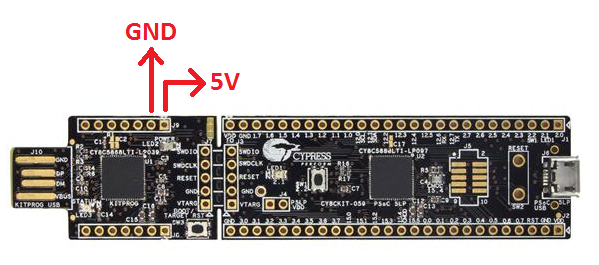
\includegraphics[width=4in]{psoc}
	\caption{PSoC boards. }
	\label{fig:psoc}
\end{figure}
